The notch in the specular direction can be thought of as arising from 
interference between the specularly reflected beam and the
re-radiated SPP field which is antiphase at $\theta_\mathrm{SP}$.  There
is, however, an additional important signature which can be observed in the
same half-space.  During propagation, roughness or other surface
inhomogenities can elastically modify the in-plane momentum of an SPP.
This is known as ``directional scattering'', the signature of which is a
annular cone of light at $\theta_\mathrm{SP}$ along an azimuthal coordinate
$\phi$.  The coordinates of this light and its relationship to the specular
notch are depicted in \Figure{fig:conefig}.  In our 
discussions, we will use the term ``cone'' when refering to light scattered
into the cone, and ``notch'' when refering to light in the specular
direction.
\begin{figure}[ht]
 \centering
 \import{includes/}{setpgfinc}
 %\import{existence/figures/}{conefig}
 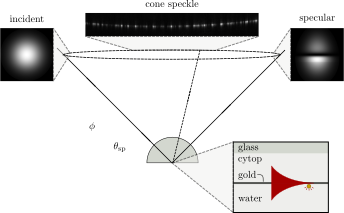
\includegraphics{existence/figures/conefig}
 \caption{Coordinates of the conically scattered light in relation to the
 prism, incident, and specular reflected beams.}
 \label{fig:conefig}
\end{figure}

Physically, the mechanism describing this phenomena proceeds as follows:
light first transmits the prism and permeates the metal film, exciting
SPPs.  We identifiy this by the Fresnel \textit{forward}
transmission coefficent, $t^p_+$ (e.g. for a three layer system with layers
0, 1, and 2, $t^p_+ \equiv t^p_{012}$).  Upon re-radiation as a photon, the
light will take this path in reverse, which we identify by the Fresnel
\textit{reverse} transmission, $t^p_-$ (e.g. $t^p_- \equiv t^p_{210}$).  We
define intensity in the cone $I_\mathrm{cone}$ as proportional to the
product of these two~\cite{simon1976directional}.
\begin{equation}
I_\mathrm{cone} 
= \frac{1}{I_0}\frac{\mathrm{d}I}{\mathrm{d}\Omega} 
= 4 \left(\frac{\omega}{c}\right)^4 |t^p_+|^2
|t^p_-|^2\,W(\theta_i,\theta_s,\phi)\, |s(\Delta \mathbf{k})|^2
\label{eqn:guhacone}
\end{equation}
where $I_0$ is the incident power, $\mathrm{d}I/\mathrm{d}\Omega$ is the
scattered power per solid angle, $s(\Delta \mathbf{k})$ is the surface
roughness spectrum, and $W(\theta_i,\theta_s,\phi)$ \textit{describes the
								interference of the two roughness induced current components in the
plane of incidence}.

\begin{equation}
|s(\Delta \mathbf{k})|^2 = \frac{\sigma^2}{4\pi} \left<S^2\right>
\me^{-(\Delta k^2 \sigma^2)/4}
\label{eqn:surfaceroughness}
\end{equation}

Whatever, some roughness stuff, I just say the following:
\begin{equation}
|E_\mathrm{cone}|^2 \propto	|t^p_+|^2 |t^p_-|^2
\label{eqn:conefield}
\end{equation}

Due to the double enhancement factor in \Equation{eqn:guhacone}, light in
the cone has a narrower linewidth than its specular counterpart in the
notch.  In \Figure{fig:conevsnotch} we show a simulated provfile of the
normalized and inverted cone vs notch for a three layer system
($n_1=1.5142$, $n_2=\num{0.2843 + 3.3825i}$, $n_3=1.331$ and
$d_2=\SI{45}{\nano\meter}$).  This aspect causes certain measurements in
the cone to be more sensitive than those in the notch, an aspect we will
visit in \Chapter{ch:bulkri}.
\begin{figure}[ht]
 \centering
 \import{includes/}{setpgfinc}
 \import{existence/figures/}{cone_vs_notch}
 \caption{Comparison of the angular profiles of the cone and notch.  The
	cone has been inverted and normalized to the same range as the notch for
	comparison.}
 \label{fig:conevsnotch}
\end{figure}

Finally, something about speckle and how we'll talk about it later.

Look what I have done!
